\documentclass{standalone}
\usepackage{tikz}
\usetikzlibrary{patterns, positioning}


\begin{document}
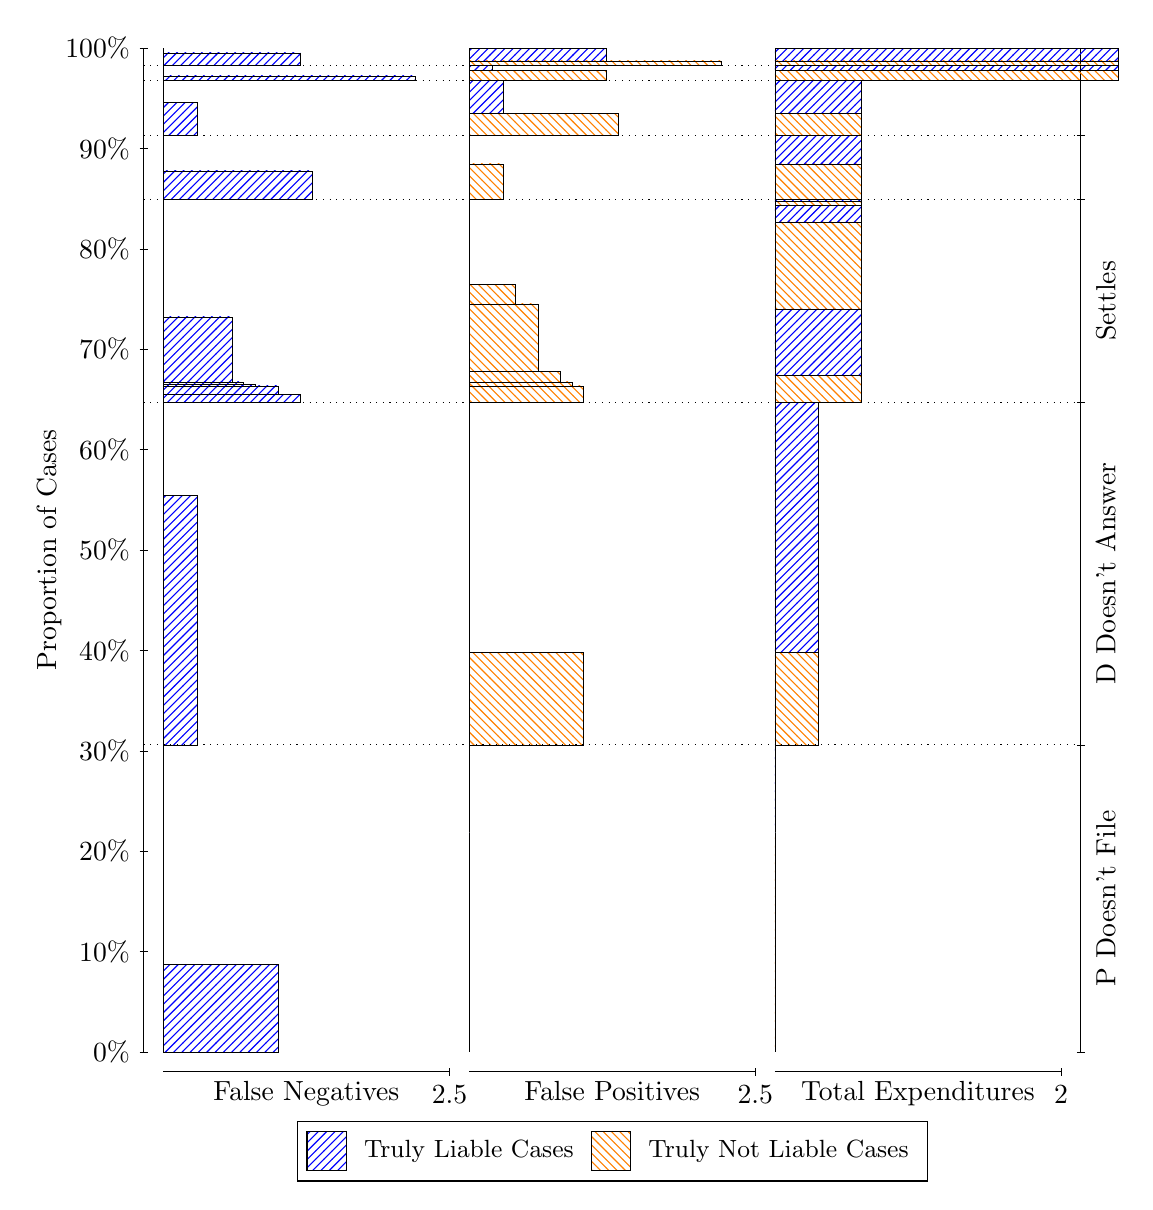
\begin{tikzpicture}
\draw[black, very thin] (1.5,1.75) -- (1.5,14.5);
\node[rotate=90, text=black, anchor=center] at (0.3, 8.125) {Proportion of Cases};
\draw[black, very thin] (1.45,1.75) -- (1.55,1.75);
\node[text=black, anchor=east] at (1.45, 1.75) {0\%};
\draw[black, very thin] (1.45,3.025) -- (1.55,3.025);
\node[text=black, anchor=east] at (1.45, 3.025) {10\%};
\draw[black, very thin] (1.45,4.3) -- (1.55,4.3);
\node[text=black, anchor=east] at (1.45, 4.3) {20\%};
\draw[black, very thin] (1.45,5.575) -- (1.55,5.575);
\node[text=black, anchor=east] at (1.45, 5.575) {30\%};
\draw[black, very thin] (1.45,6.85) -- (1.55,6.85);
\node[text=black, anchor=east] at (1.45, 6.85) {40\%};
\draw[black, very thin] (1.45,8.125) -- (1.55,8.125);
\node[text=black, anchor=east] at (1.45, 8.125) {50\%};
\draw[black, very thin] (1.45,9.4) -- (1.55,9.4);
\node[text=black, anchor=east] at (1.45, 9.4) {60\%};
\draw[black, very thin] (1.45,10.675) -- (1.55,10.675);
\node[text=black, anchor=east] at (1.45, 10.675) {70\%};
\draw[black, very thin] (1.45,11.95) -- (1.55,11.95);
\node[text=black, anchor=east] at (1.45, 11.95) {80\%};
\draw[black, very thin] (1.45,13.225) -- (1.55,13.225);
\node[text=black, anchor=east] at (1.45, 13.225) {90\%};
\draw[black, very thin] (1.45,14.5) -- (1.55,14.5);
\node[text=black, anchor=east] at (1.45, 14.5) {100\%};

\draw[black, very thin] (13.4,1.75) -- (13.4,14.5);
\draw[black, very thin] (13.35,1.75) -- (13.45,1.75);
\node[anchor=west] at (13.35, 1.75) {};
\draw[black, very thin] (13.35,5.6496) -- (13.45,5.6496);
\node[anchor=west] at (13.35, 5.6496) {};
\draw[black, very thin] (13.35,10.001) -- (13.45,10.001);
\node[anchor=west] at (13.35, 10.001) {};
\draw[black, very thin] (13.35,12.578) -- (13.45,12.578);
\node[anchor=west] at (13.35, 12.578) {};
\draw[black, very thin] (13.35,13.393) -- (13.45,13.393);
\node[anchor=west] at (13.35, 13.393) {};
\draw[black, very thin] (13.35,14.086) -- (13.45,14.086);
\node[anchor=west] at (13.35, 14.086) {};
\draw[black, very thin] (13.35,14.276) -- (13.45,14.276);
\node[anchor=west] at (13.35, 14.276) {};
\draw[black, very thin] (13.35,14.5) -- (13.45,14.5);
\node[anchor=west] at (13.35, 14.5) {};

\draw[black, very thin, pattern color=blue, pattern=north east lines] (1.75,1.75) rectangle (3.2033,2.8608);
\draw[black, very thin, pattern color=orange, pattern=north west lines] (1.75,2.8608) rectangle (1.75,5.6496);
\draw[black, very thin, pattern color=blue, pattern=north east lines] (1.75,5.6496) rectangle (2.186,8.8215);
\draw[black, very thin, pattern color=orange, pattern=north west lines] (1.75,8.8215) rectangle (1.75,10.001);
\draw[black, very thin, pattern color=blue, pattern=north east lines] (1.75,10.001) rectangle (3.494,10.102);
\draw[black, very thin, pattern color=blue, pattern=north east lines] (1.75,10.102) rectangle (3.2033,10.209);
\draw[black, very thin, pattern color=blue, pattern=north east lines] (1.75,10.209) rectangle (2.9127,10.233);
\draw[black, very thin, pattern color=blue, pattern=north east lines] (1.75,10.233) rectangle (2.7673,10.261);
\draw[black, very thin, pattern color=blue, pattern=north east lines] (1.75,10.261) rectangle (2.622,11.085);
\draw[black, very thin, pattern color=orange, pattern=north west lines] (1.75,11.085) rectangle (1.75,12.578);
\draw[black, very thin, pattern color=blue, pattern=north east lines] (1.75,12.578) rectangle (3.6393,12.941);
\draw[black, very thin, pattern color=orange, pattern=north west lines] (1.75,12.941) rectangle (1.75,13.393);
\draw[black, very thin, pattern color=blue, pattern=north east lines] (1.75,13.393) rectangle (2.186,13.814);
\draw[black, very thin, pattern color=orange, pattern=north west lines] (1.75,13.814) rectangle (1.75,14.086);
\draw[black, very thin, pattern color=blue, pattern=north east lines] (1.75,14.086) rectangle (4.9473,14.147);
\draw[black, very thin, pattern color=orange, pattern=north west lines] (1.75,14.147) rectangle (1.75,14.276);
\draw[black, very thin, pattern color=blue, pattern=north east lines] (1.75,14.276) rectangle (3.494,14.439);
\draw[black, very thin, pattern color=orange, pattern=north west lines] (1.75,14.439) rectangle (1.75,14.5);
\draw[black, very thin, pattern color=orange, pattern=north west lines] (5.6333,1.75) rectangle (5.6333,4.5388);
\draw[black, very thin, pattern color=blue, pattern=north east lines] (5.6333,4.5388) rectangle (5.6333,5.6496);
\draw[black, very thin, pattern color=orange, pattern=north west lines] (5.6333,5.6496) rectangle (7.0867,6.8289);
\draw[black, very thin, pattern color=blue, pattern=north east lines] (5.6333,6.8289) rectangle (5.6333,10.001);
\draw[black, very thin, pattern color=orange, pattern=north west lines] (5.6333,10.001) rectangle (7.0867,10.208);
\draw[black, very thin, pattern color=orange, pattern=north west lines] (5.6333,10.208) rectangle (6.9413,10.259);
\draw[black, very thin, pattern color=orange, pattern=north west lines] (5.6333,10.259) rectangle (6.796,10.389);
\draw[black, very thin, pattern color=orange, pattern=north west lines] (5.6333,10.389) rectangle (6.5053,11.252);
\draw[black, very thin, pattern color=orange, pattern=north west lines] (5.6333,11.252) rectangle (6.2147,11.494);
\draw[black, very thin, pattern color=blue, pattern=north east lines] (5.6333,11.494) rectangle (5.6333,12.578);
\draw[black, very thin, pattern color=orange, pattern=north west lines] (5.6333,12.578) rectangle (6.0693,13.03);
\draw[black, very thin, pattern color=blue, pattern=north east lines] (5.6333,13.03) rectangle (5.6333,13.393);
\draw[black, very thin, pattern color=orange, pattern=north west lines] (5.6333,13.393) rectangle (7.5227,13.666);
\draw[black, very thin, pattern color=blue, pattern=north east lines] (5.6333,13.666) rectangle (6.0693,14.086);
\draw[black, very thin, pattern color=orange, pattern=north west lines] (5.6333,14.086) rectangle (7.3773,14.215);
\draw[black, very thin, pattern color=blue, pattern=north east lines] (5.6333,14.215) rectangle (5.924,14.276);
\draw[black, very thin, pattern color=orange, pattern=north west lines] (5.6333,14.276) rectangle (8.8307,14.336);
\draw[black, very thin, pattern color=blue, pattern=north east lines] (5.6333,14.336) rectangle (7.3773,14.5);
\draw[black, very thin, pattern color=orange, pattern=north west lines] (9.5167,1.75) rectangle (9.5167,4.5388);
\draw[black, very thin, pattern color=blue, pattern=north east lines] (9.5167,4.5388) rectangle (9.5167,5.6496);
\draw[black, very thin, pattern color=orange, pattern=north west lines] (9.5167,5.6496) rectangle (10.062,6.8289);
\draw[black, very thin, pattern color=blue, pattern=north east lines] (9.5167,6.8289) rectangle (10.062,10.001);
\draw[black, very thin, pattern color=orange, pattern=north west lines] (9.5167,10.001) rectangle (10.607,10.338);
\draw[black, very thin, pattern color=blue, pattern=north east lines] (9.5167,10.338) rectangle (10.607,11.186);
\draw[black, very thin, pattern color=orange, pattern=north west lines] (9.5167,11.186) rectangle (10.607,12.291);
\draw[black, very thin, pattern color=blue, pattern=north east lines] (9.5167,12.291) rectangle (10.607,12.5);
\draw[black, very thin, pattern color=orange, pattern=north west lines] (9.5167,12.5) rectangle (10.607,12.55);
\draw[black, very thin, pattern color=blue, pattern=north east lines] (9.5167,12.55) rectangle (10.607,12.578);
\draw[black, very thin, pattern color=orange, pattern=north west lines] (9.5167,12.578) rectangle (10.607,13.03);
\draw[black, very thin, pattern color=blue, pattern=north east lines] (9.5167,13.03) rectangle (10.607,13.393);
\draw[black, very thin, pattern color=orange, pattern=north west lines] (9.5167,13.393) rectangle (10.607,13.666);
\draw[black, very thin, pattern color=blue, pattern=north east lines] (9.5167,13.666) rectangle (10.607,14.086);
\draw[black, very thin, pattern color=orange, pattern=north west lines] (9.5167,14.086) rectangle (13.877,14.215);
\draw[black, very thin, pattern color=blue, pattern=north east lines] (9.5167,14.215) rectangle (13.877,14.276);
\draw[black, very thin, pattern color=orange, pattern=north west lines] (9.5167,14.276) rectangle (13.877,14.336);
\draw[black, very thin, pattern color=blue, pattern=north east lines] (9.5167,14.336) rectangle (13.877,14.5);
\draw[black, dotted] (1.5,5.6496) -- (13.4,5.6496);
\draw[black, dotted] (1.5,10.001) -- (13.4,10.001);
\draw[black, dotted] (1.5,12.578) -- (13.4,12.578);
\draw[black, dotted] (1.5,13.393) -- (13.4,13.393);
\draw[black, dotted] (1.5,14.086) -- (13.4,14.086);
\draw[black, dotted] (1.5,14.276) -- (13.4,14.276);
\draw[black, very thin] (1.75,1.5) -- (5.3833,1.5);
\node[text=black, anchor=north] at (3.5667, 1.5) {False Negatives};
\draw[black, very thin] (5.3833,1.45) -- (5.3833,1.55);
\node[text=black, anchor=north] at (5.3833, 1.45) {2.5};

\draw[black, very thin] (5.6333,1.5) -- (9.2667,1.5);
\node[text=black, anchor=north] at (7.45, 1.5) {False Positives};
\draw[black, very thin] (9.2667,1.45) -- (9.2667,1.55);
\node[text=black, anchor=north] at (9.2667, 1.45) {2.5};

\draw[black, very thin] (9.5167,1.5) -- (13.15,1.5);
\node[text=black, anchor=north] at (11.333, 1.5) {Total Expenditures};
\draw[black, very thin] (13.15,1.45) -- (13.15,1.55);
\node[text=black, anchor=north] at (13.15, 1.45) {2};

\node[text=black, centered, rotate=90] at (13.72, 3.6998) {P Doesn't File};
\node[text=black, centered, rotate=90] at (13.72, 7.8252) {D Doesn't Answer};
\node[text=black, centered, rotate=90] at (13.72, 11.289) {Settles};





\draw (7.449999999999999,1.5) node[draw=none] (baseCoordinate) {};
\begin{scope}[align=center]
        \matrix[scale=0.5, draw=black, below=0.5cm of baseCoordinate, nodes={draw}, column sep=0.1cm]{
            \node[rectangle, draw, minimum width=0.5cm, minimum height=0.5cm, pattern color=blue, pattern=north east lines] {}; &
            \node[draw=none, font=\small, text=black] (B) {Truly Liable Cases}; &
            \node[rectangle, draw, minimum width=0.5cm, minimum height=0.5cm, pattern color=orange, pattern=north west lines] {}; &
            \node[draw=none, font=\small, text=black] (B) {Truly Not Liable Cases}; \\
            };
\end{scope}

\end{tikzpicture}
\end{document}